\documentclass[10pt]{beamer}
\usetheme{Boadilla}
\usepackage[utf8]{inputenc}
\usepackage{amsmath}
\usepackage{amsfonts}
\usepackage{amssymb}
\usepackage{graphicx}
\author{Adriano Del Vincio}
\title{Studying Annihilation Distributions}
%\setbeamercovered{transparent} 
%\setbeamertemplate{navigation symbols}{} 
\logo{
\includegraphics[width = 0.125\textwidth]{../logo/logounibs.png}} 
%\institute{} 
%\date{} 
%\subject{} 
\begin{document}

\begin{frame}
\titlepage
\end{frame}

%\begin{frame}
%\tableofcontents
%\end{frame}

\begin{frame}{}

I tried to fit the distributions of the event annihilation with analytic models. This should improve the results, avoiding statistical fluctuations:
The models are listed below:
\begin{itemize}
\item Pdf Mixing: the Normal distribution.
\item Pdf Uwlosses: Rayleigh distribution $\frac{r}{\sigma^{2}} e^{-\frac{r^{2}}{2 \sigma^{2}}}$.
\item Pdf Cosmic: $\frac{1}{8} x$.
\end{itemize}

The factor $\frac{1}{8}$ for the cosmic is due to normalization. The Mixing, UW losses and cosmic data are fitted and the result are shown in the following slides 
\end{frame}

\begin{frame}{MIXING}

\begin{figure}
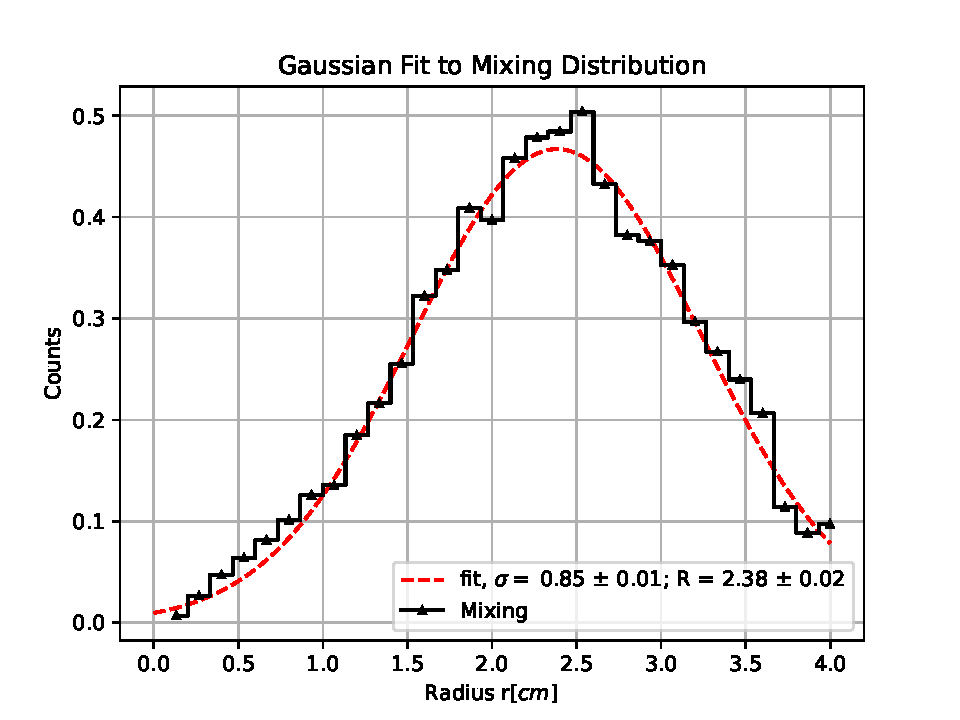
\includegraphics[width = 0.8\textwidth]{GaussianFitMixing.pdf}
\end{figure}

\end{frame}

\begin{frame}{UWlosses}

\begin{figure}
\includegraphics[width = 0.75\textwidth]{FitToUW.pdf}
\end{figure}

\end{frame}

\begin{frame}{Cosmic}

\begin{figure}
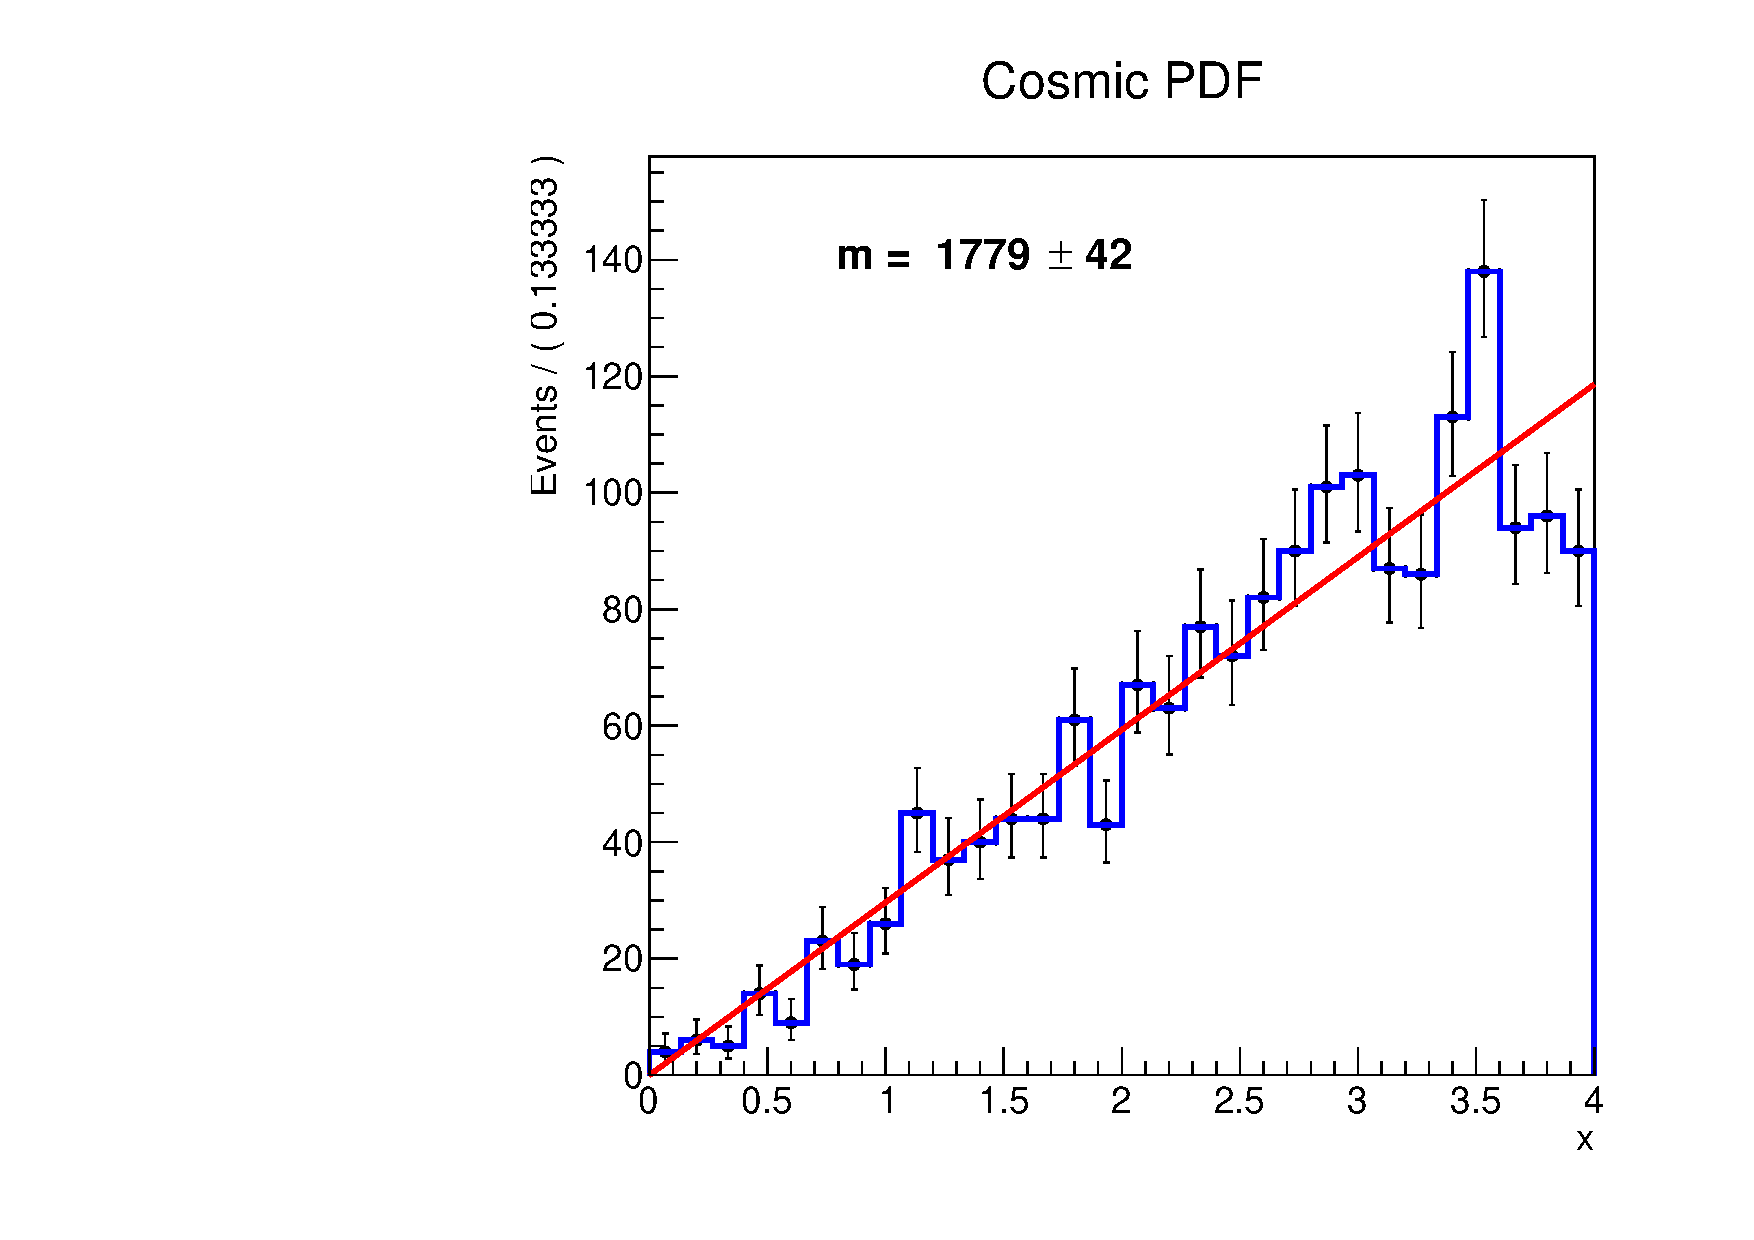
\includegraphics[width = 0.7\textwidth]{Cosmici_fit.pdf}
\end{figure}

\end{frame}

\begin{frame}{Pdfs normalized plotted together}
\begin{figure}
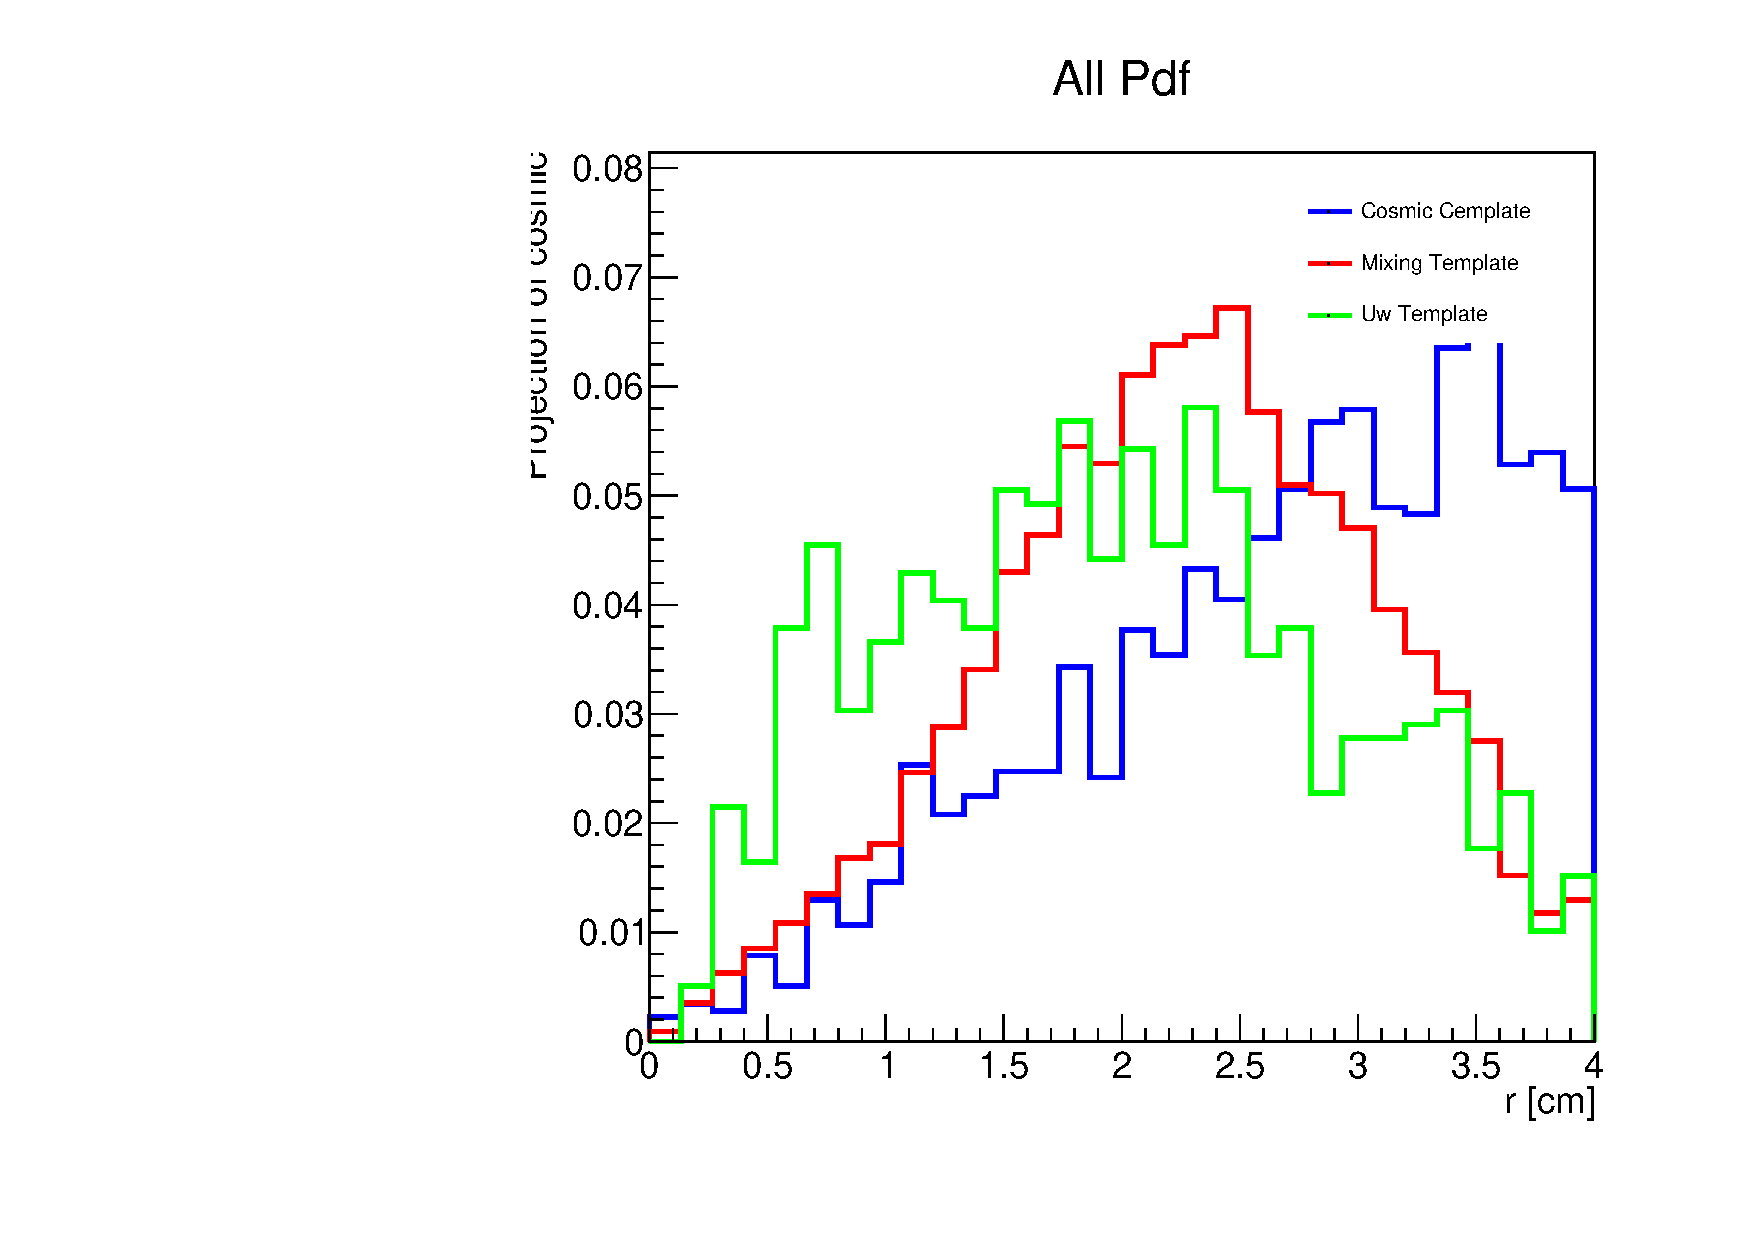
\includegraphics[width = 0.80\textwidth]{PdfTogether.pdf}
\end{figure}
\end{frame}

\begin{frame}{Pdf with radius normalization}

The histogram in $r$ variable doesn't account for the different area of the bin which is $2 \pi r \cdot dr$. So it is useful to normalize dividing per $2 \pi r$.

\begin{figure}[hbtp]
\centering
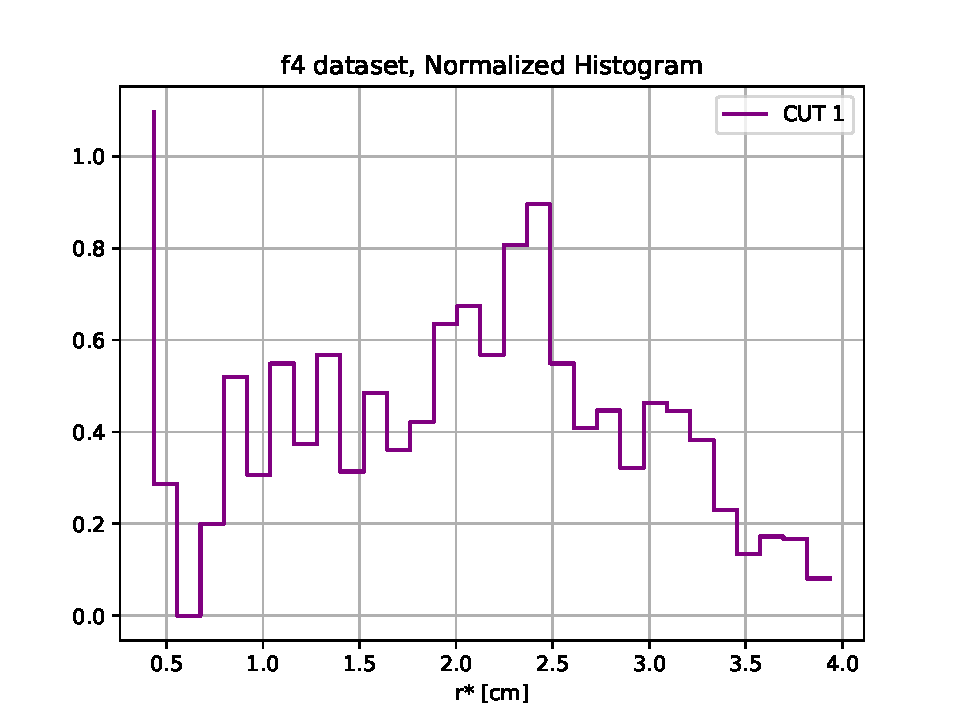
\includegraphics[width = 0.8\textwidth]{Normalizedf4.pdf}
\caption{Pdf normalized for f4 dataset}
\end{figure}
\end{frame}

\begin{frame}{Pdf with radius normalization}

\begin{figure}[hbtp]
\centering
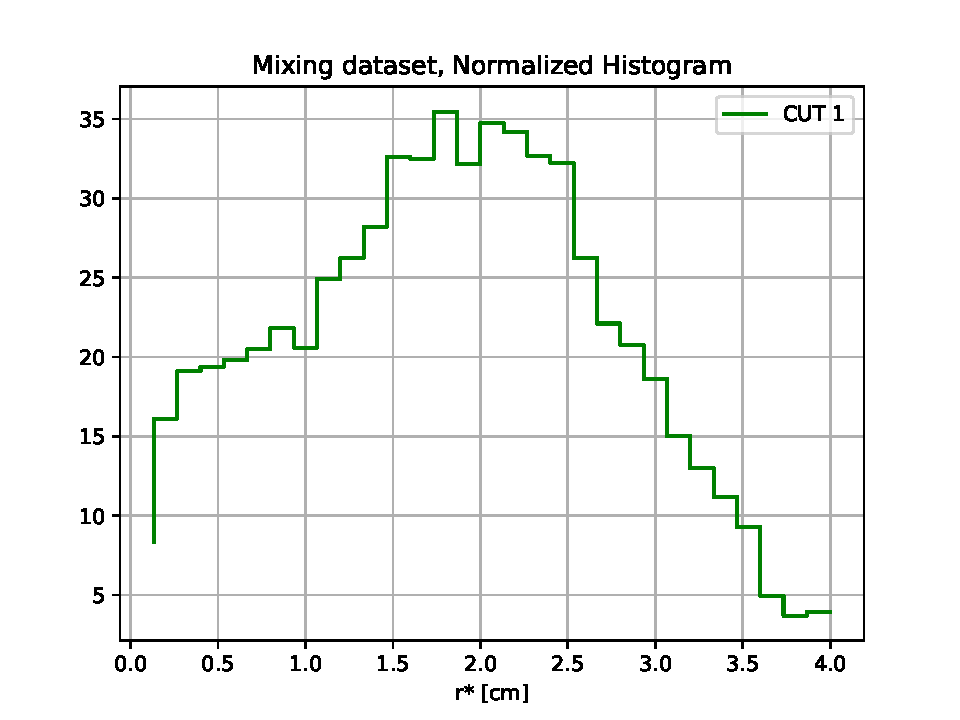
\includegraphics[width = 0.8\textwidth]{NormalizedMixing.pdf}
\caption{Pdf normalized for Mixing dataset}
\end{figure}
\end{frame}

\begin{frame}{Pdf with radius normalization}

\begin{figure}[hbtp]
\centering
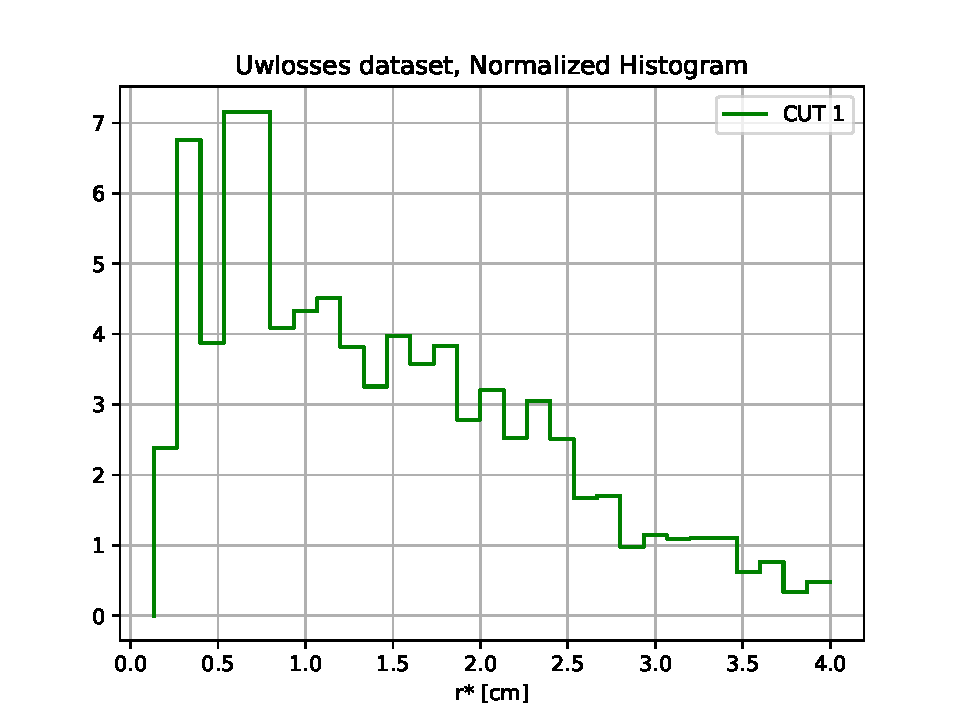
\includegraphics[width = 0.8\textwidth]{NormalizedUW.pdf}
\caption{Pdf normalized for UW dataset}
\end{figure}
\end{frame}

\begin{frame}{Pdf with radius normalization}

\begin{figure}[hbtp]
\centering
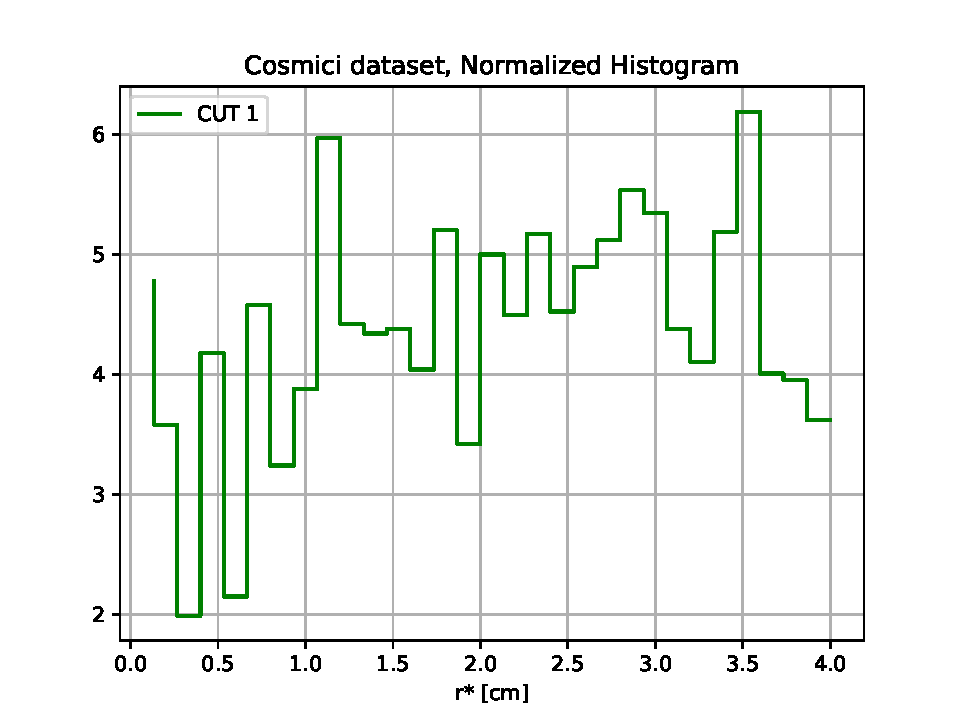
\includegraphics[width = 0.8\textwidth]{NormalizedBK.pdf}
\caption{Pdf normalized for Cosmic dataset}
\end{figure}
\end{frame}

\begin{frame}{fit with all template}

Pdf = Template Mixing + Template Uwlosses + Template cosmic

\begin{figure}[hbtp]
\centering
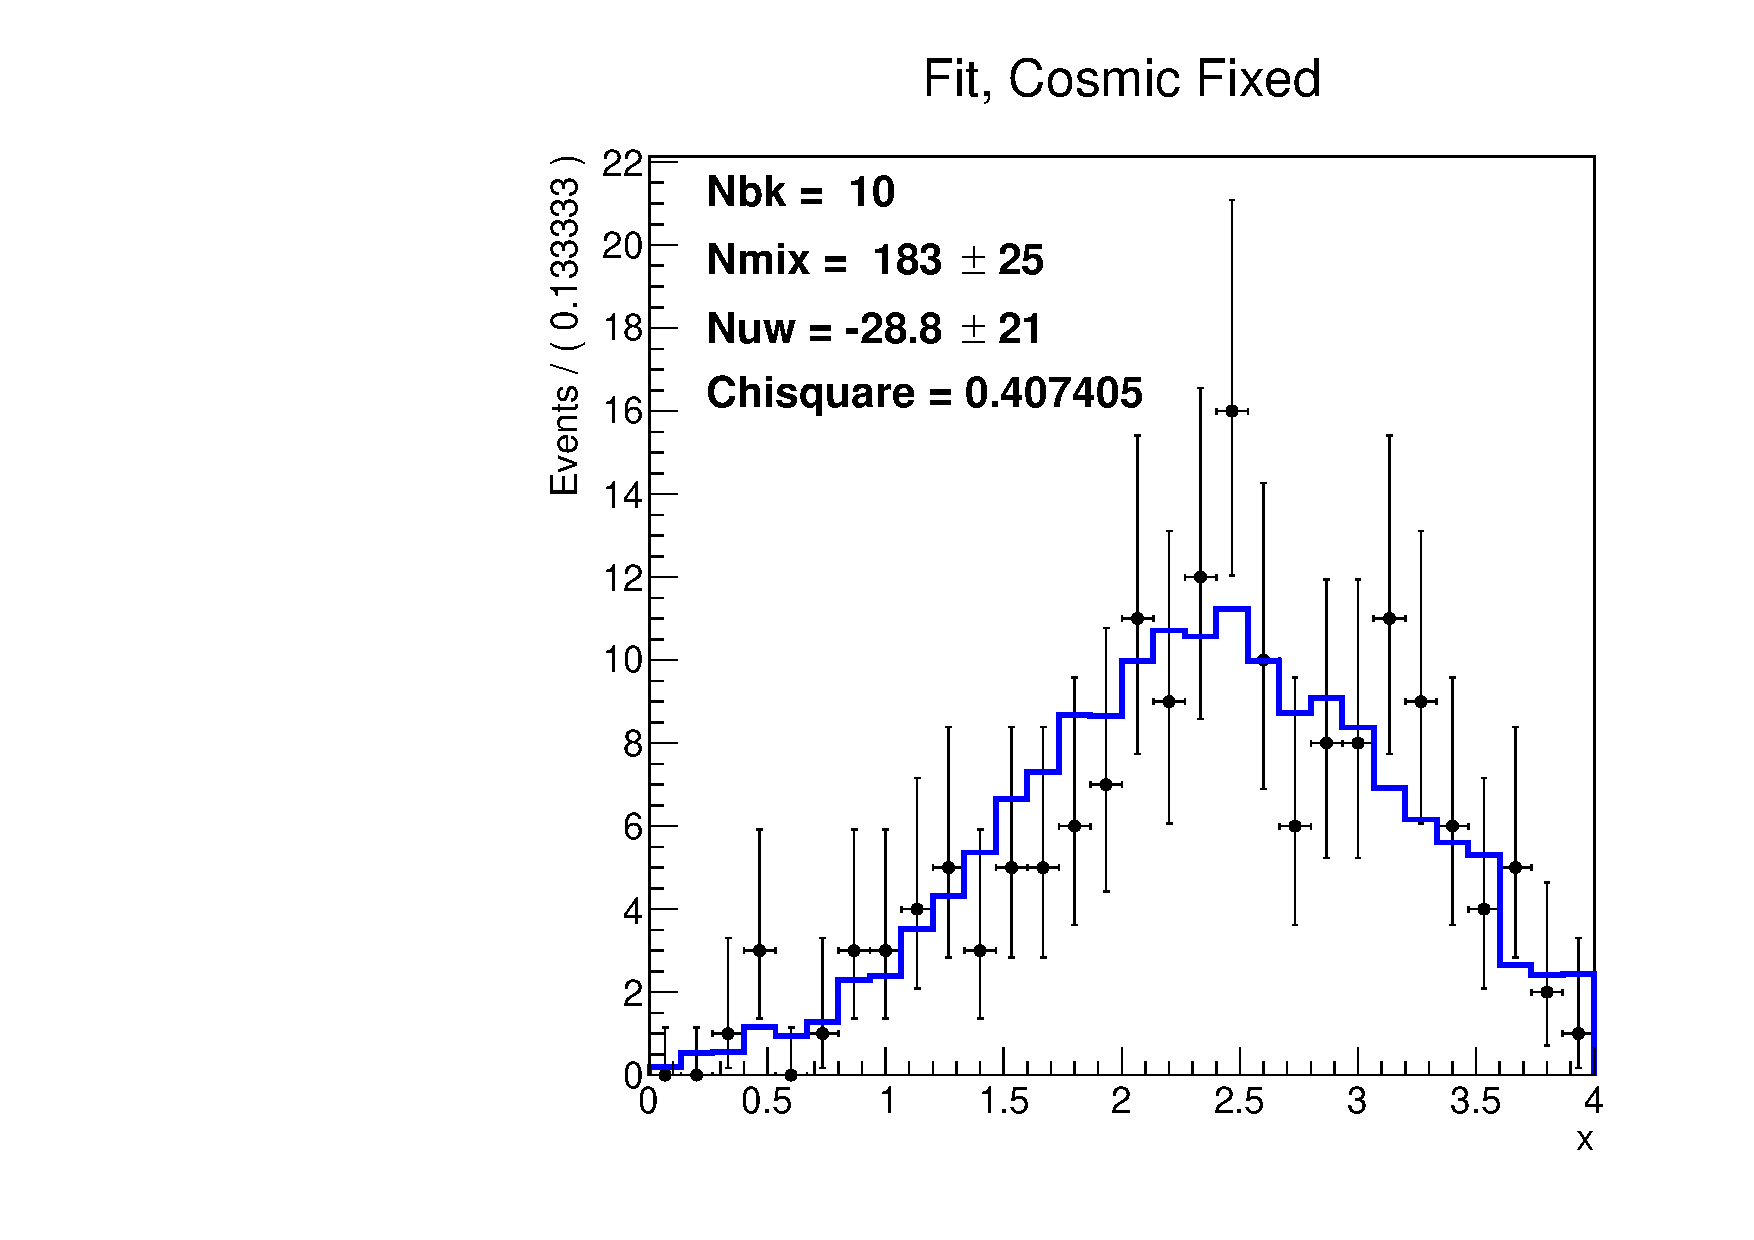
\includegraphics[width = 0.65 \textwidth]{FitTemplate.pdf}
\end{figure}
\end{frame}

\begin{frame}{fit with analytic models}

Pdf = Gaussian (Mixing) + Rayleigh (Uwlosses) + linear model (cosmic)

\begin{figure}[hbtp]
\centering
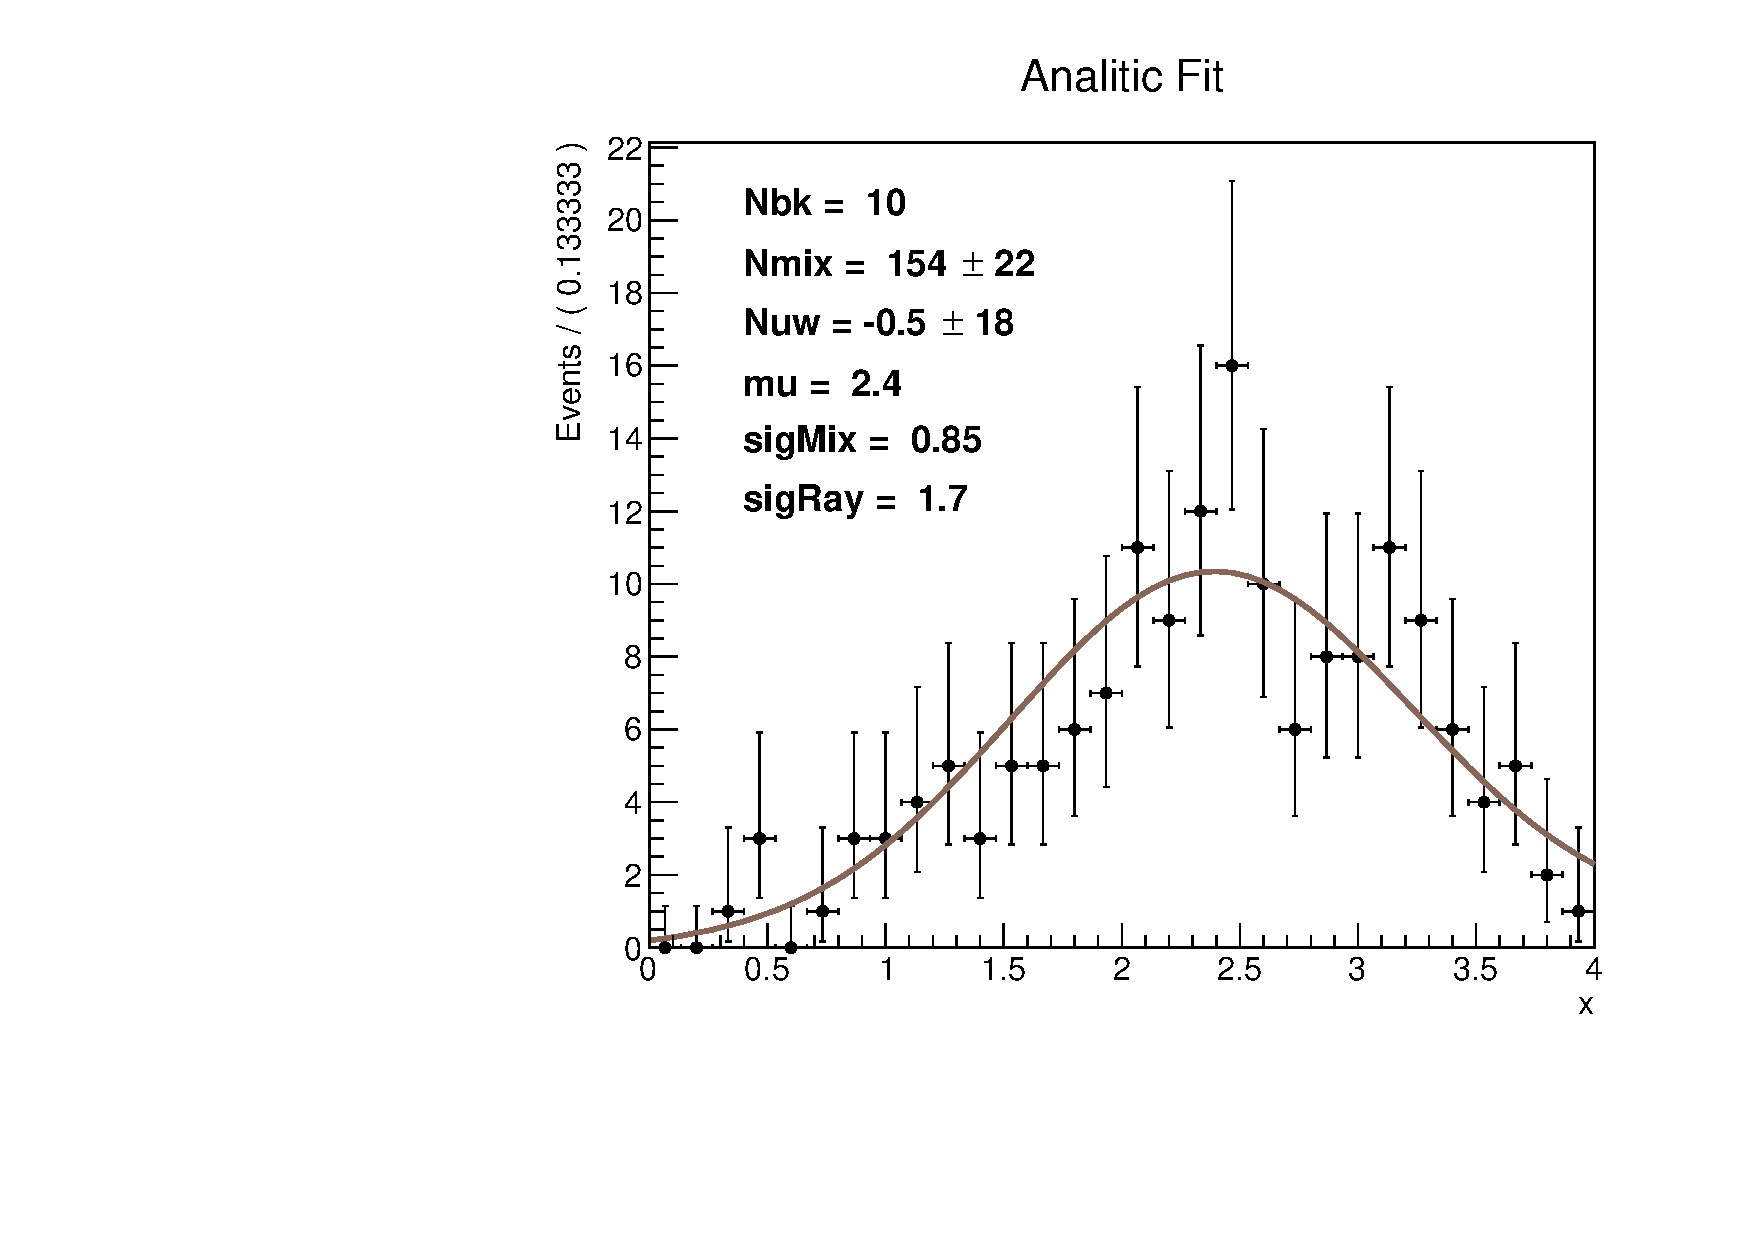
\includegraphics[width = 0.70 \textwidth]{TuttoAnalitico.pdf}
\end{figure}
\end{frame}


\begin{frame}{Montecarlo simulation}

To study the accuracy of the algorithm to reconstruct the various parameter, a "toy" algorithm is done. The model to generate the data is:

\begin{equation}
Pdf_{total} = a \cdot Template_{mix} + b \cdot Rayleigh + c \cdot linearModel_{cosmic} 
\end{equation}

$a,b,c$ represent the "weight", or degree or percentage of the various contributions to the Pdf used to generate the data. For simplicity the $c$ is setted to zero. 

We generate $N$ data. Once the data are generated, they are fitted with the model:

\begin{equation}
Pdf_{fit} = N_{mix} \cdot Template_{mix} + N_{uw} \cdot Rayleigh
\end{equation}

The parameters of the fit are $N_{mix}, N_{uw}$. The difference between the data from the fit and the "real values" is plotted. The "true value" are defined as:


\begin{itemize}
\centering
\item Nmix true $= a \cdot N$
\item Nuw true  $= b \cdot N$
\item Nbk true  $= c \cdot N$
\end{itemize} 

\end{frame}

\begin{frame} {N = 165, a = 100, b = 0, c = 0}

\begin{figure}
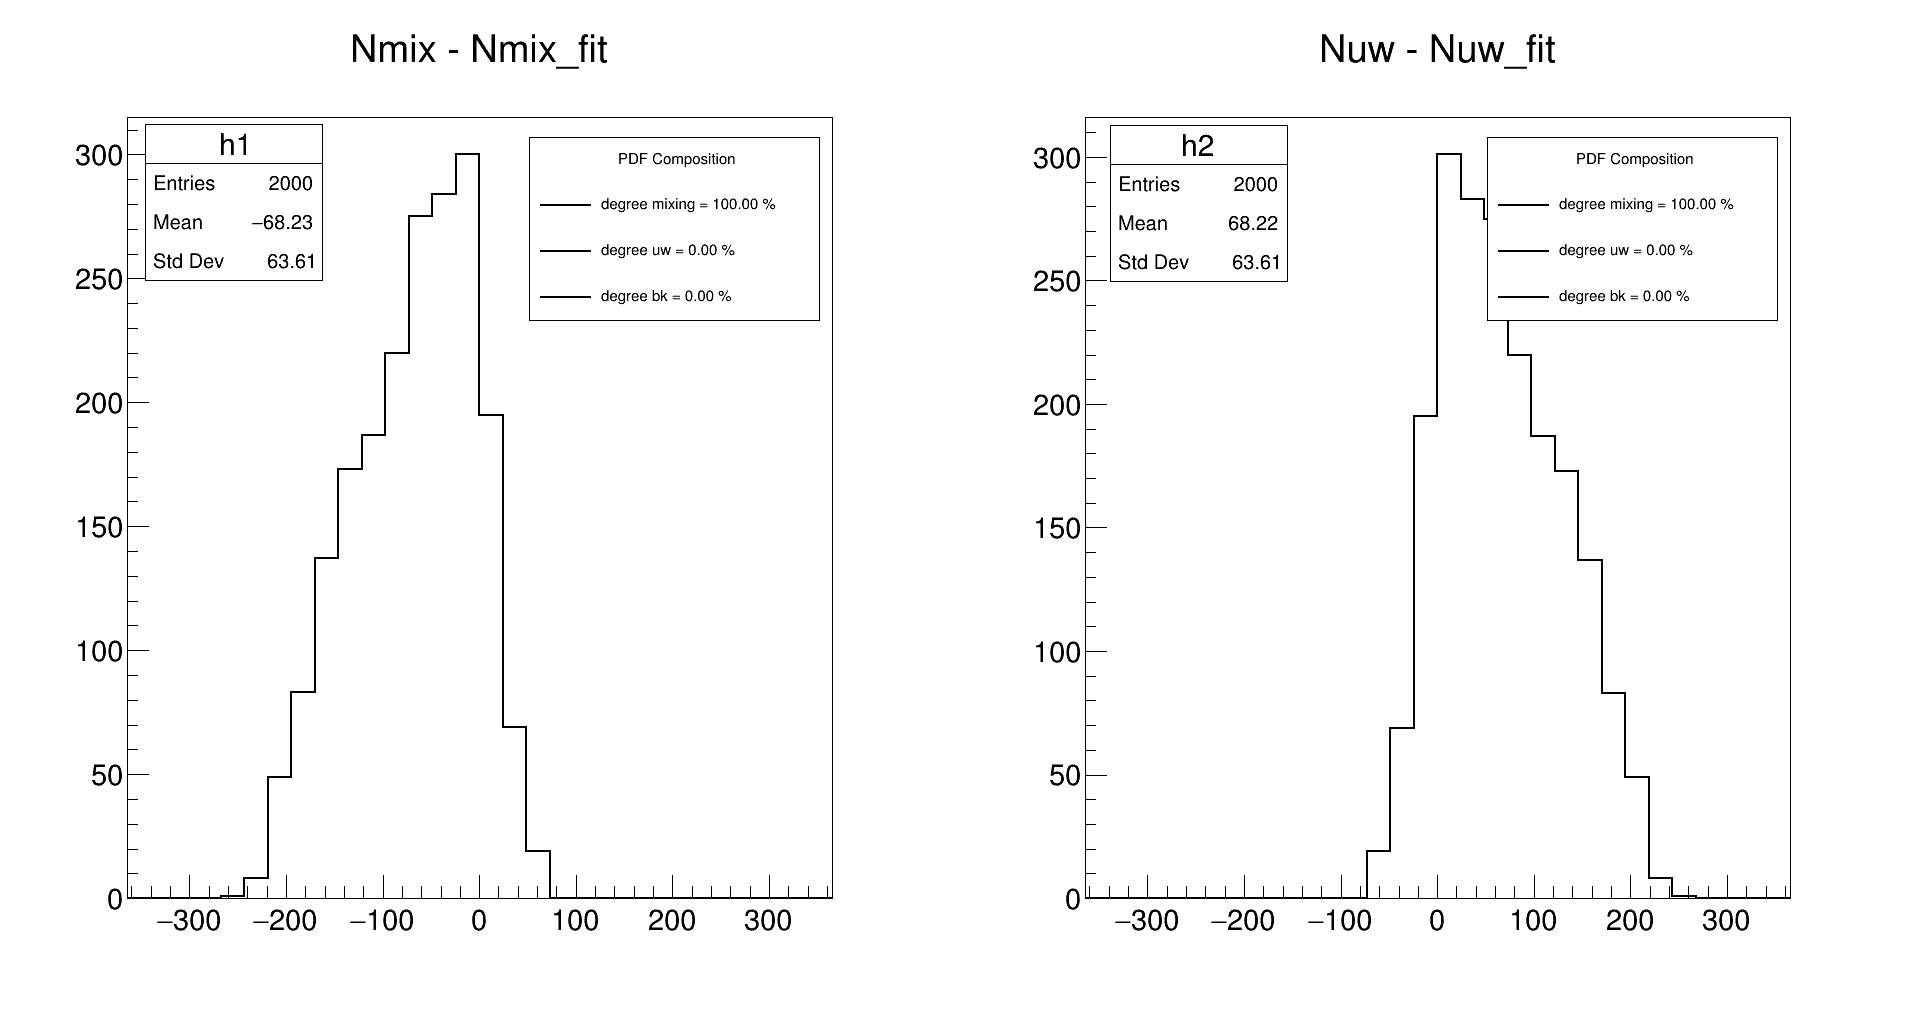
\includegraphics[width = 1\textwidth]{Nequalto164/toy(100,0,0).png} 
\end{figure}

\end{frame}

\begin{frame}{N = 165, a = 75, b = 25, c = 0}

\begin{figure}
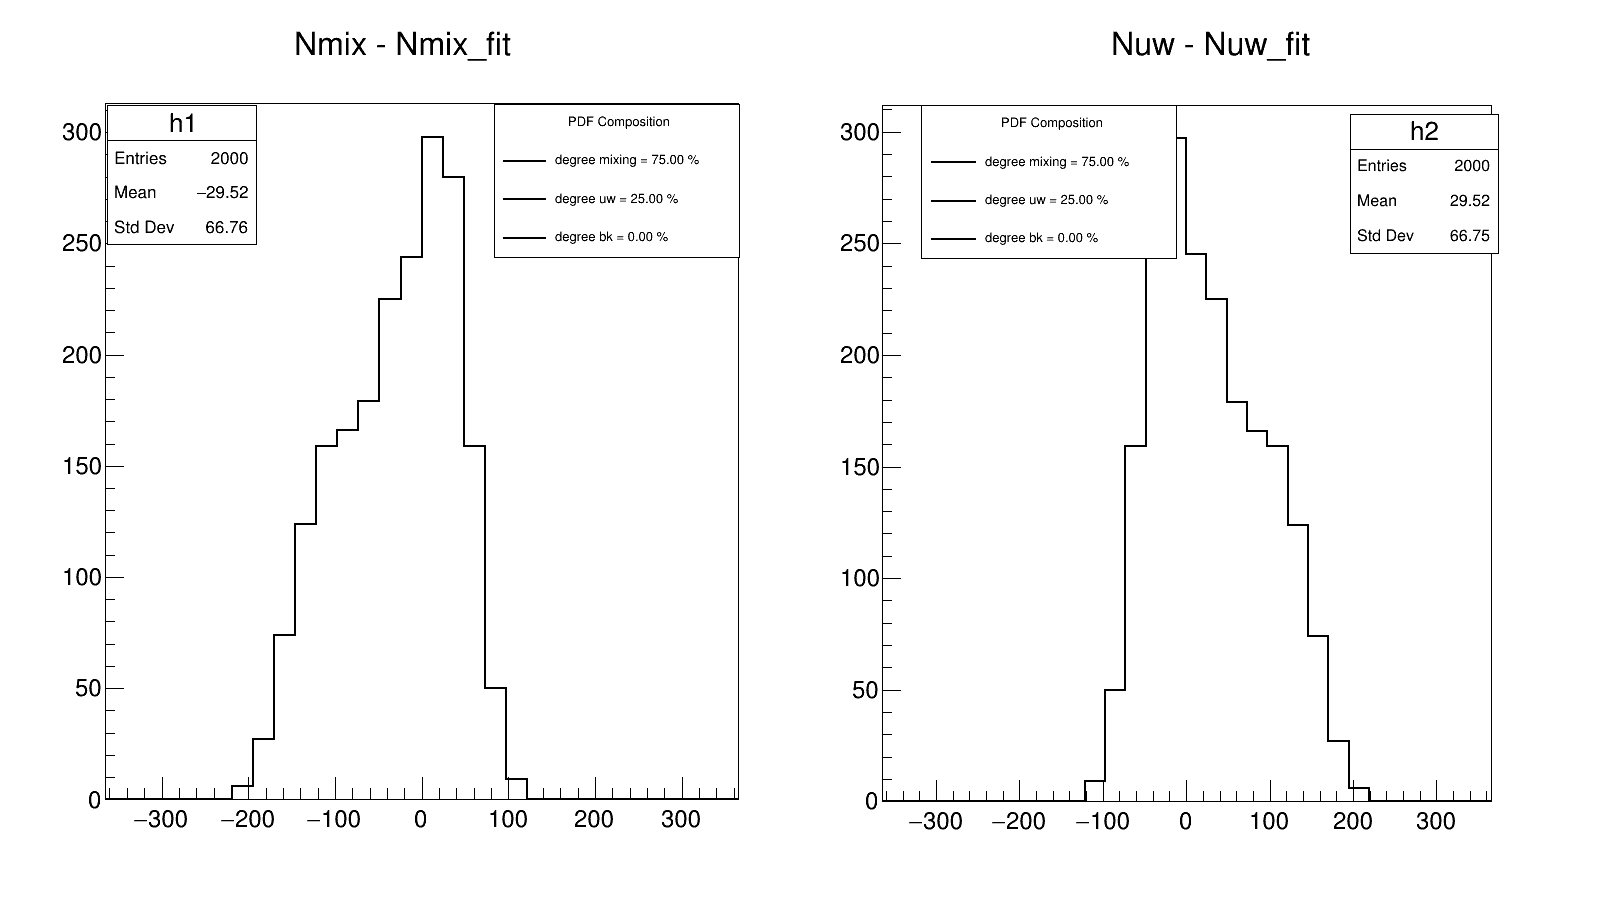
\includegraphics[width = 1\textwidth]{Nequalto164/toy(75,25,0).png} 
\end{figure}
\end{frame}

\begin{frame}{N = 165, a = 50, b = 50, c = 0}
\begin{figure}
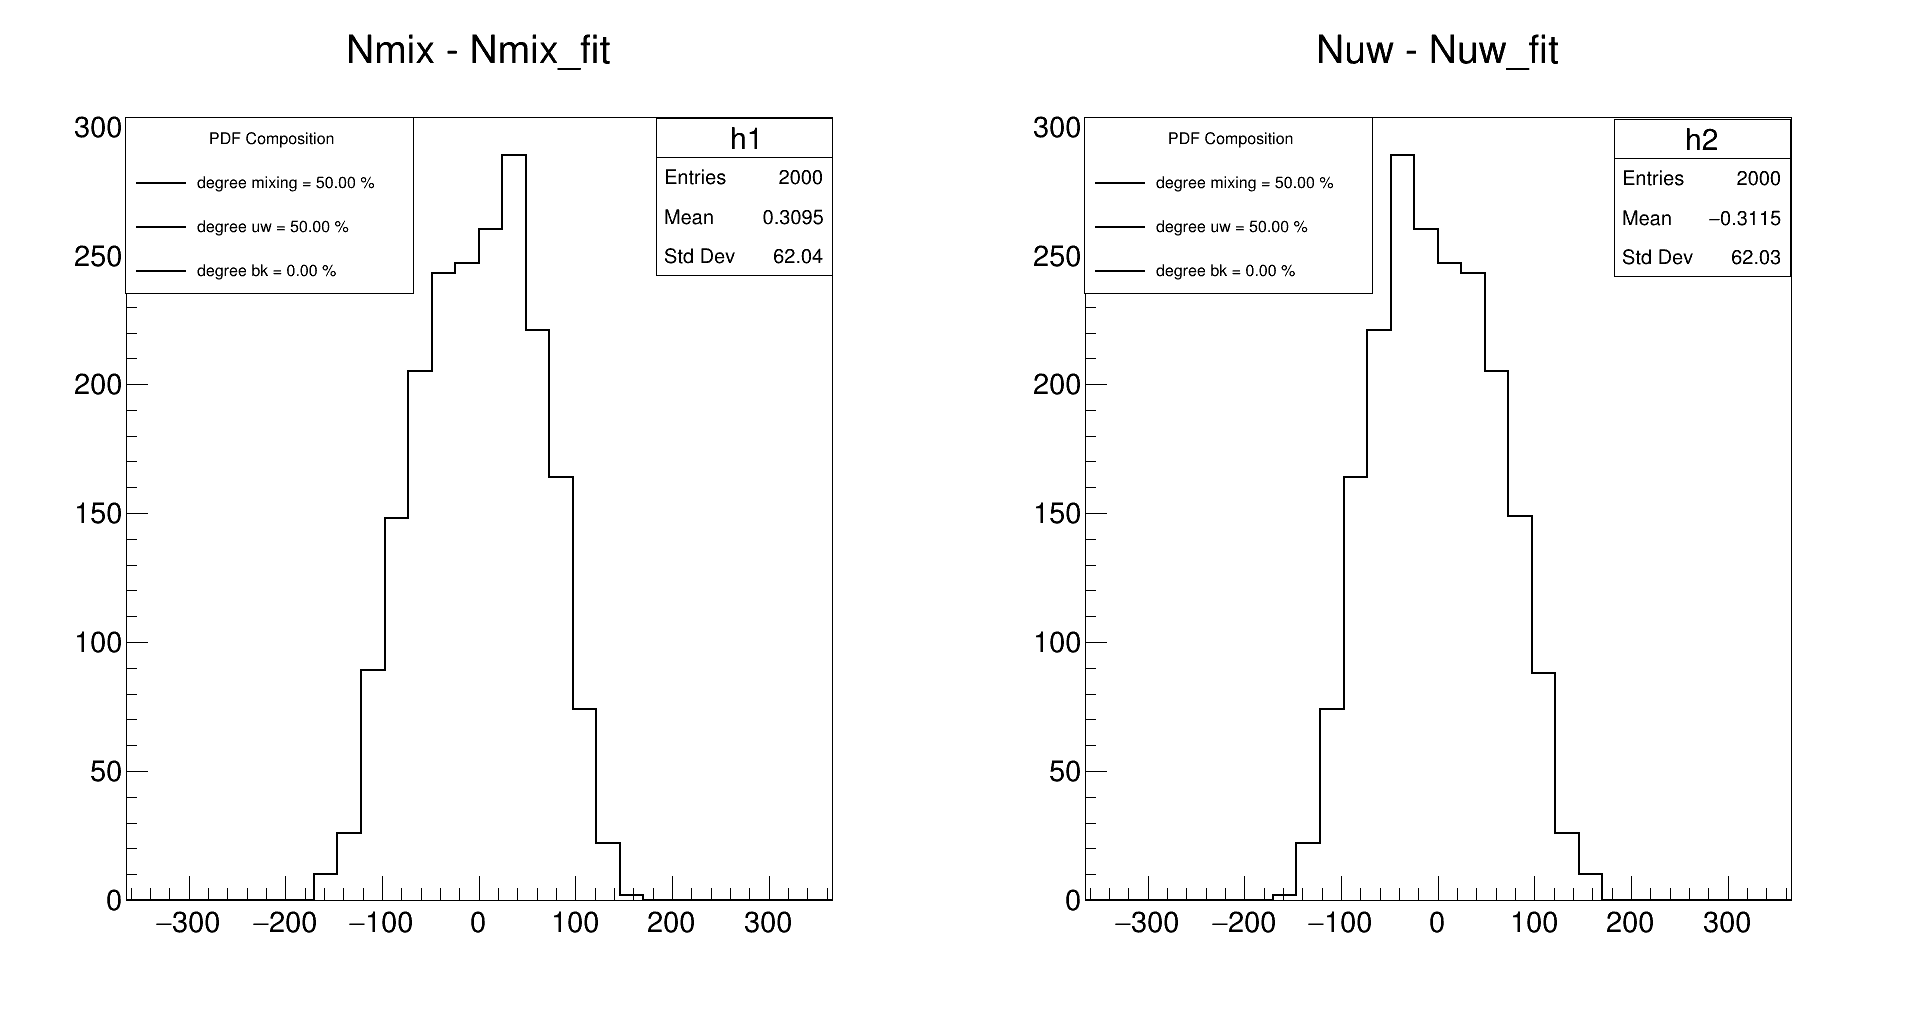
\includegraphics[width = 1\textwidth]{Nequalto164/toy(50,50,0).png}
\end{figure}
\end{frame}

\end{document}